\chapter{Nástroj pro analýzu kontraktů}
	Cílem práce z hlediska implementace bylo vytvořit nástroj, který by umožňoval získání informací o kontraktech podle výše navrženého modelu ze zdrojové či přeložené formy Java programu. Výsledná aplikace by pak měla umožnit vytvoření externí reprezentace dat a případně také porovnání DbC konstrukcí. Nástroj by měl být schopen zpracovat alespoň dva způsoby popisu DbC konstrukcí a měl by dovolovat snadné rozšíření pro další způsoby. S~využitím tohoto nástroje by pak měla být vytvořena jednoduchá uživatelská aplikace, která by sloužila k načtení a zobrazení dat modelu.\\
	
	Smyslem aplikace je umožnit detekci kontraktů ve zdrojových, respektive přeložených, souborech jazyka Java. Nalezené kontrakty je pak možné analyzovat a zkoumat způsob a četnost použití jednotlivých typů v různých projektech. Aby bylo možno získaná data dále analyzovat, je zde také export do formátu JSON. Nástroj umožňuje porovnání dvou adresářů se soubory, což může být užitečné zejména při porovnání různých verzí projektu. Můžeme tak zjistit, zda se nezměnilo rozhraní či zda se zpřísnily podmínky kontraktů oproti předchozí verzi.\\
	
	Celý nástroj je rozdělen do dvou velkých částí. První z nich je knihovna, která poskytuje všechny potřebné metody pro práci se soubory jazyka Java, jejich analýzu a zpracování, extrakci kontraktů a jejich následné porovnání a export. Druhou částí je uživatelská aplikace, která využívá metod této knihovny a umožňuje její pohodlnou obsluhu. Tento vztah je znázorněn na stručném obrázku \ref{globalArchitecture}. Na obrázku \ref{componentDiagram} je pak vidět komponentový diagram, který obsahuje více podrobností.
					
	\begin{figure}[!htb]
		\minipage{1\textwidth}	
			\centering
			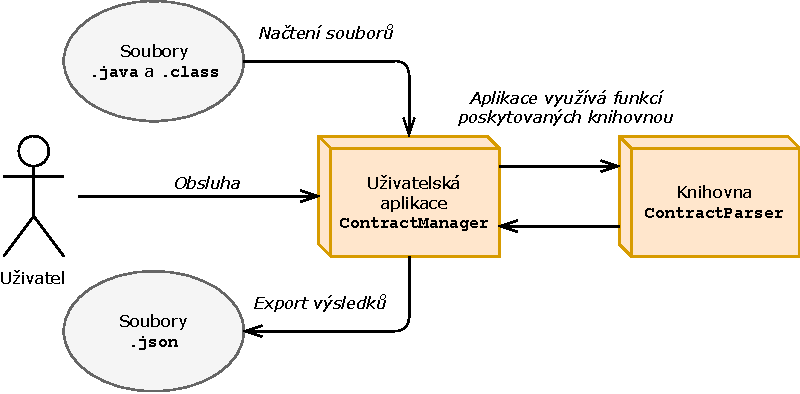
\includegraphics{img/globalArchitecture.pdf}
			\caption[globalArchitecture]{Stručná architektura nástroje}
			\label{globalArchitecture}
		\endminipage\hfill
	\end{figure}
	
	\begin{figure}[!htb]
		\minipage{1\textwidth}	
			\centering
			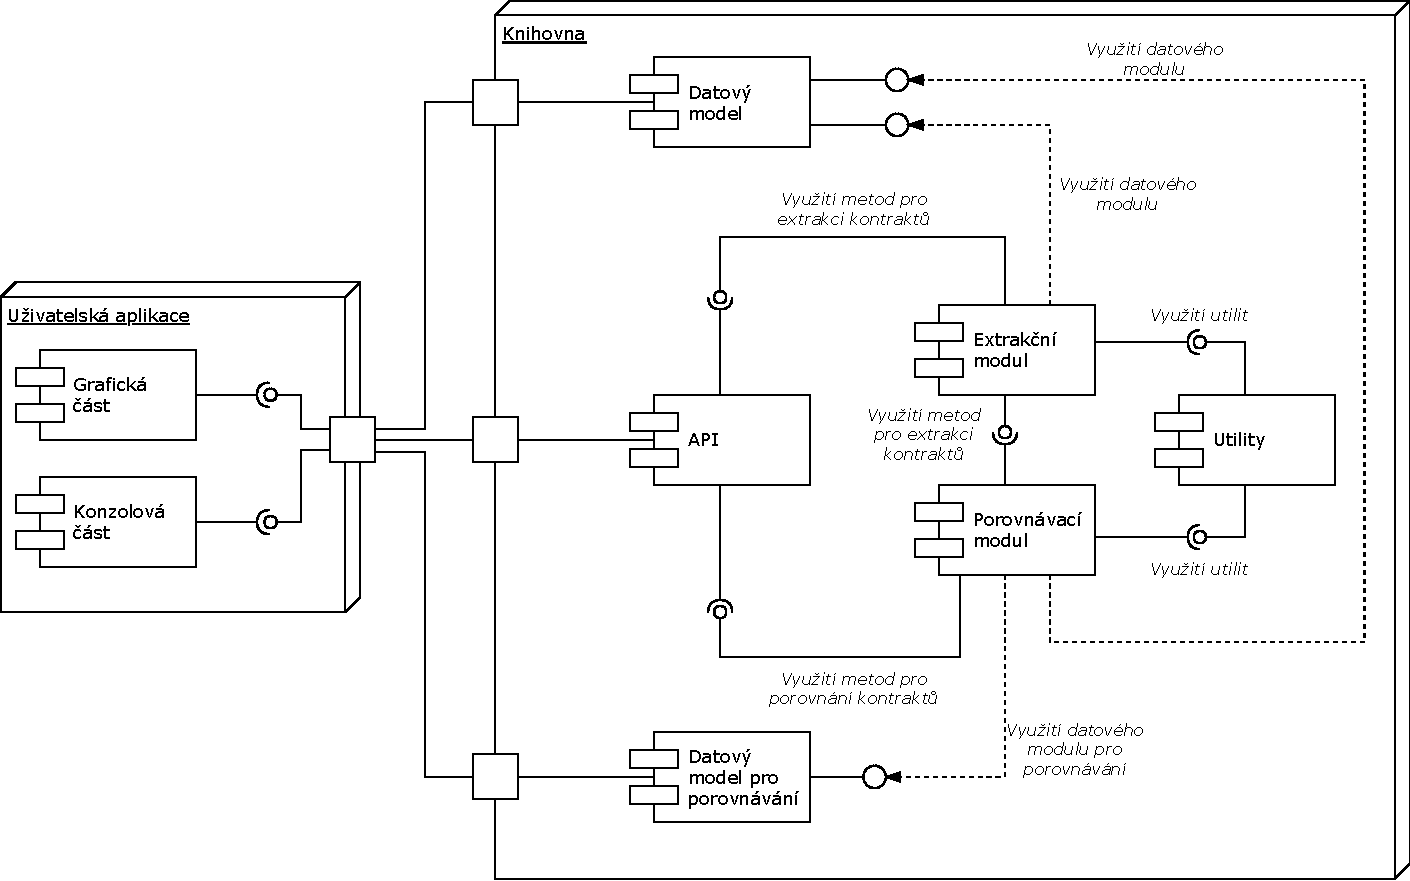
\includegraphics[width=1\textwidth]{img/componentDiagram.pdf}
			\caption[componentDiagram]{Komponentový diagram nástroje}
			\label{componentDiagram}
		\endminipage\hfill
	\end{figure}		
	
%%%%%%%%%%%%%%%%%%%%%%%%%%%%%%%%%%%%%%%%%%%%%%%%%%%%%%%%%%%%%%%%%%%%%%%%%%%%%%%%%%%%%%%%%%%%%%%%%%%%%%%%%%%%%%%%%%%%%%%%%%%%%%%%%%%%%%%%%%%%%%%%%%%%%%%%%%%%%%%%%%%%%%%%%%%%%%%%%%%%%%%%
%%%%%%%%%%%%%%%%%%%%%%%%%%%%%%%%%%%%%%%%%%%%%%%%%%%%%%%%%%%%%%%%%%%%%%%%%%%%%%%%%%%%%%%%%%%%%%%%%%%%%%%%%%%%%%%%%%%%%%%%%%%%%%%%%%%%%%%%%%%%%%%%%%%%%%%%%%%%%%%%%%%%%%%%%%%%%%%%%%%%%%%%
%%%%%%%%%%%%%%%%%%%%%%%%%%%%%%%%%%%%%%%%%%%%%%%%%%%%%%%%%%%%%%%%%%%%%%%%%%%%%%%%%%%%%%%%%%%%%%%%%%%%%%%%%%%%%%%%%%%%%%%%%%%%%%%%%%%%%%%%%%%%%%%%%%%%%%%%%%%%%%%%%%%%%%%%%%%%%%%%%%%%%%%%
%%%%%%%%%%%%%%%%%%%%%%%%%%%%%%%%%%%%%%%%%%%%%%%%%%%%%%%%%%%%%%%%%%%%%%%%%%%%%%%%%%%%%%%%%%%%%%%%%%%%%%%%%%%%%%%%%%%%%%%%%%%%%%%%%%%%%%%%%%%%%%%%%%%%%%%%%%%%%%%%%%%%%%%%%%%%%%%%%%%%%%%%
	\section{Knihovna}
		Pro realizace nástroje jsem se rozhodl implementovat knihovnu, která poskytuje metody potřebné pro extrakci, porovnání a export kontraktů. Její součástí je také model použitý pro jejich reprezentaci. 

%%%%%%%%%%%%%%%%%%%%%%%%%%%%%%%%%%%%%%%%%%%%%%%%%%%%%%%%%%%%%%%%%%%%%%%%%%%%%%%%%%%%%%%%%%%%%%%%%%%%%%%%%%%%%%%%%%%%%%%%%%%%%%%%%%%%%%%%%%%%%%%%%%%%%%%%%%%%%%%%%%%%%%%%%%%%%%%%%%%%%%%%	
	    \subsection{Použité technologie}
	    
	    	\subsubsection{Programovací jazyk}
				Pro tvorbu knihovny jsem použil jazyk Java verze 1.8. Jedním z hlavních důvodů bylo, že nástroj zkoumá reprezentace kontraktů v jazyce Java, díky tomu je možné dané konstrukce snadno testovat a zkoušet přímo v tomto projektu. Vedoucí práce také upřednostňoval použití jazyka Java z důvodů případného propojení s jinými nástroji, které byly vyvinuty pro práci s kontrakty v rámci univerzity a jsou také realizovány v Java. Osobně mám s jazykem Java pravděpodobně největší zkušenosti, což byl další z důvodů, proč tento jazyk použít. Díky těmto okolnostem byla volba jazyka poměrně jednoznačná.\\
				
				I přesto, že v průběhu vývoje projektu vyšla verze Java 1.9 a posléze i 1.10, rozhodl jsem se po domluvě s vedoucím práce ponechat stabilní verzi 1.8 a nepřecházet v průběhu vývoje na novější verzi jazyka.
				
			\subsubsection{Vývojové prostředí}				
				Nástroj byl realizován ve vývojovém prostředí IDEA IntelliJ Ultimate 2017.3.3.
	    	
			\subsubsection{Práce se závislostmi}
				Pro zajištění závislostí jako jsou knihovny třetích stran, ale také pro snadnou distribuci knihovny, jsem zvolil technologii Apache Maven \cite{maven}. Jedná se o široce používaný nástroj pro získávání závislostí a tvorbu projektů.
				
			\subsubsection{Logování}
				Pro logování, tedy zobrazení a uložení chybových či informačních zpráv, byla použita knihovna Apache Log4j \cite{log4j}. Tato knihovna umožňuje pokročilé možnosti logování, které je možné dobře nastavit pomocí konfiguračních souborů. Opět se jedná o široce používanou technologii.
				
			\subsubsection{Tokenizace zdrojových souborů jazyka Java}
				Pro implementaci tokenizace souborů jsem se rozhodl použít knihovnu JavaParser \cite{javaparser}. Učinil jsem tak na základě mého průzkumu (viz 4. kapitola Tokenizace jazyka Java). Knihovna poskytuje komplexní reprezentaci daného zdrojového souboru a je tak možné jej dále analyzovat a zpracovávat. Knihovnu je možné snadno použít přímo v projektu díky zprostředkovanému API.
			
			\subsubsection{Dekompilace přeložených souborů jazyka Java}
				Jako dekompilátor přeložených souborů jazyka Java (\texttt{.class}) jsem použil knihovnu Procyon \cite{procyon}. Jedná se o nástroj, který umožňuje snadnou dekompilaci souborů a to včetně moderních konstrukcí jazyka Java. Hlavním důvodem volby této knihovny byla možnost použití dekompilace v rámci kódu za pomocí API. Více informací je opět k dispozici ve 4. kapitole.
				
			\subsubsection{Práce s formátem JSON}
				Pro ukládání reprezentací do formátu JSON byla použita knihovna Gson \cite{gson}. Umožňuje intuitivní převod objektu typu Java\footnote{Mohou být použity téměř libovolné objekty, avšak nesmějí být cyklické (Objekt nesmí ve své hierarchii atributů opět obsahovat tentýž objekt)} do formátu JSON za pomocí API. Mimo jiné také umožňuje formátování \emph{Pretty Print}, které je lépe čitelné pro člověka.
				
			\subsubsection{Testování}
				Pro tvorbu jednotkových testů byla použita technologie jUnit 5 \cite{junit}.   	 


%%%%%%%%%%%%%%%%%%%%%%%%%%%%%%%%%%%%%%%%%%%%%%%%%%%%%%%%%%%%%%%%%%%%%%%%%%%%%%%%%%%%%%%%%%%%%%%%%%%%%%%%%%%%%%%%%%%%%%%%%%%%%%%%%%%%%%%%%%%%%%%%%%%%%%%%%%%%%%%%%%%%%%%%%%%%%%%%%%%%%%%%	

		\subsection{Návrh nástroje}
			Celý nástroj je rozdělen do několika modulů, viz obrázek \ref{componentDiagram}. Oba datové modely byly popsaný výše v 5. kapitole. Parsovací modul je klíčovou součástí celého nástroje. Umožňuje zpracování kódu jazyka Java a jeho analýzu. Poskytuje prostředky pro uležení tohoto analyzovaného kódu do navržené struktury a následnou extrakci kontraktů. Porovnávací modul umožňuje porovnávání složek a souborů z hlediska kontraktů a API. Utility poskytují metody pro práci se zdroji a soubory. API je navržena pro snadné vnější použití celé knihovny. Jednotlivé moduly jsou popsány níže.		
		
				
%%%%%%%%%%%%%%%%%%%%%%%%%%%%%%%%%%%%%%%%%%%%%%%%%%%%%%%%%%%%%%%%%%%%%%%%%%%%%%%%%%%%%%%%%%%%%%%%%%%%%%%%%%%%%%%%%%%%%%%%%%%%%%%%%%%%%%%%%%%%%%%%%%%%%%%%%%%%%%%%%%%%%%%%%%%%%%%%%%%%%%%%

		\subsection{Parsovací modul}
			Tento modul zajišťuje zpracování zdrojových souborů jazyka Java a následné uložení do reprezentace \texttt{ExtendedJavaFile}. To má na starosti třída \texttt{JavaFileParser}, která také využívá třídy \texttt{MethodVisitor}. Pokud je vstupní soubor typu \texttt{.class} je nejprve dekompilován. Dekompilaci, stejně tak jako ostatní práci se soubory, zajišťuje třída \texttt{IOServices} (viz níže).\\
			
			Třída \texttt{ExtendedJavaFile} je součástí modelu pro parsování, který dědí od svých rodičovských tříd ze základního datového modelu výše (zde konkrétně je děděno od třídy \texttt{JavaFile}). Dále je zde třída \texttt{ExtendedJavaClass} a \texttt{ExtendedJavaMethod}. Tento rozšířený model ukládá dodatečné informace jako je tělo metod, anotace atd. Z těchto informací jsou následně získávány kontrakty.\\
			
			Vytvořená struktura je následně procházena a jsou z ní extrahovány kontrakty. To zajišťují třídy \texttt{GuavaParser} a \texttt{JSR305Parser} (každá svůj cílený typ kontraktu). Tyto třídy implementují rozhraní \texttt{ContractParser} a továrna \texttt{ParserFactory} umožňuje vytváření jejich instancí. Tímto způsobem se instance objektu \texttt{ExtendedJavaFile} postupně rozšiřuje.\\
			
			Poté co byly extrahovány všechny kontrakty, podrobnosti o metodách a třídách jsou již redundantní a z toho důvodu je objekt \texttt{ExtendedJavaFile} zredukován na \texttt{JavaFile}. Totéž platí pro zbytek modelu. K této redukci slouží třída \texttt{Simplifier}.\\
			
			Poslední částí tohoto modulu je třída \texttt{ContractExtractor}. Ta slouží jako výchozí bod pro komunikaci s ostatními částmi nástroje a spojuje dílčí třídy a jejich funkce dohromady. V podstatě se jedná o API pro vnitřní užití knihovny.\\
			
			Graficky je možné vidět tento modul v podobě UML diagramu, který je zobrazen na obrázku \ref{parserUMLdiagram}. Jedná se o zjednodušený UML diagram tříd, kde jsou jednotlivé metody omezeny pouze na svůj název a návratovou hodnotu. Důvodem je to, že metody mají mnoho vstupních parametrů, což by činilo diagram nepřehledný. Podrobnosti o konkrétních třídách je pak možné získat z JavaDoc dokumentace (na CD ve složce \texttt{javaDoc}). Rozšíření model je také zjednodušen a jsou zde zobrazeny pouze atributy, které nemají rodičovské třídy zobrazené v modelu výše. K datovému modelu je také přistupováno jako k celku, aby se zmenšilo množství závislostních vazeb (mnoho tříd pracuje s většinou částí modelu). V projektu je pak modul reprezentován balíčkem \texttt{parser}\\
			
			Základní pracovní postup pro extrakci kontraktů je možné vidět na obrázku \ref{workFlow}. Jedná se o jednoduchý diagram, který slouží jako grafický podklad k popisu jednotlivých činností a jejich návazností. Diagram slouží pouze pro rychlou orientaci a přehled v procesu, proto tu nejsou znázorněny nestandardní aktivity jako zpracování chyb atd.

				\begin{figure}[!htb]
					\minipage{1\textwidth}	
						\centering
						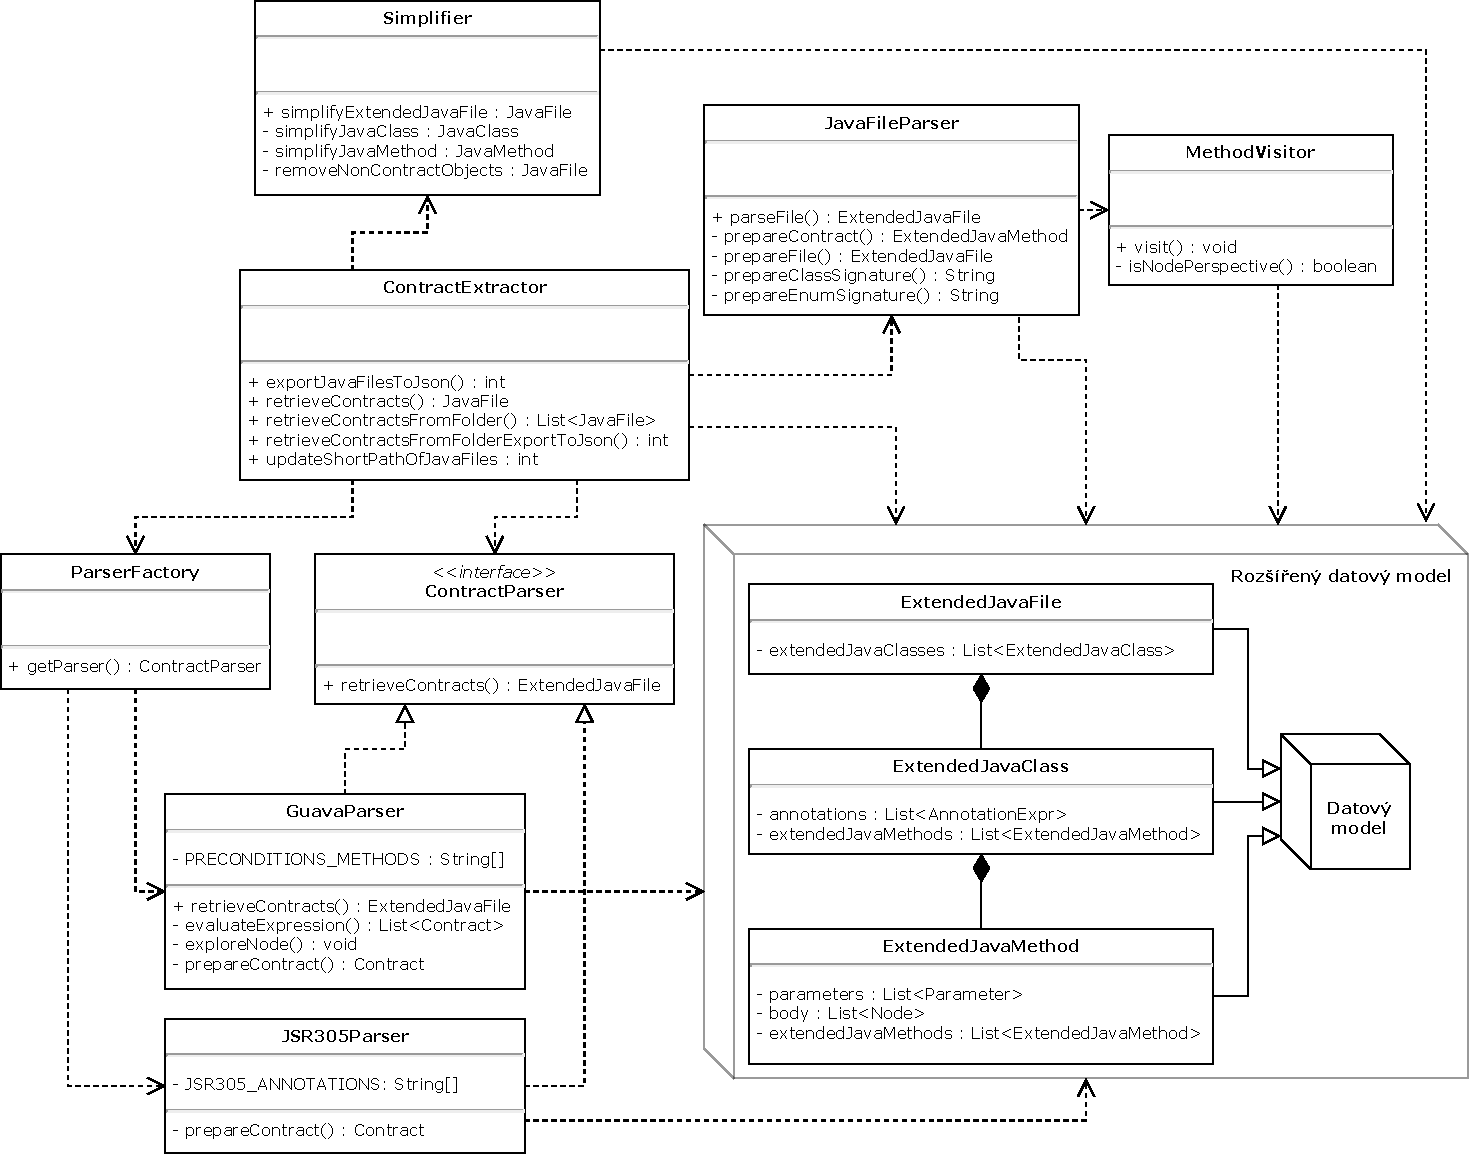
\includegraphics[width=1\textwidth]{img/parserUMLdiagram.pdf}
						\caption[parserUMLdiagram]{UML diagram parsovacího modulu}
						\label{parserUMLdiagram}
					\endminipage\hfill
				\end{figure}
			
				\begin{figure}[!htb]
					\minipage{1\textwidth}	
						\centering
						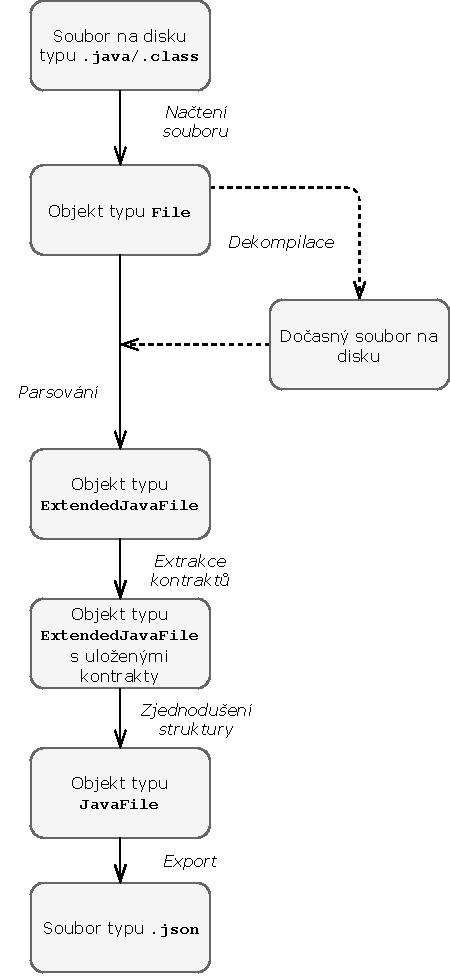
\includegraphics{img/workFlow.pdf}
						\caption[workFlow]{Základní pracovní postup}
						\label{workFlow}
					\endminipage\hfill
				\end{figure}
		
			\subsubsection{Parsování Java souborů}	    
				Pro zpracování zdrojových souborů jazyku Java byla použita knihovna JavaParser. Ta poskytuje metodu \texttt{parse()}, která vytvoří komplexní strukturu daného zdrojového souboru. V prvním kroku se tato struktura projde a vyhledá všechny třídy (\emph{class}) a také rozhraní \emph{interface} a výčtové typy \emph{enum}. Pro účely modelu jsou si tyto tři prvky rovny. Každý nalezený prvek je následně uložen do modelu. V případě třídy a rozhraní se struktura prochází dále a do modelu jsou uloženy všechny konstruktory, které se z hlediska modelu považují za metody (viz níže). Následně jsou uloženy všechny anotace dané \uv{třídy}.\\
			
				Po této přípravě je využita třída \texttt{MethodVisitor}, která dědí od třídy \texttt{VoidVisitorAdapter} a umožňuje procházet všechny metody v daném souboru. V metodě pak máme k dispozici objekt typu \texttt{MethodDeclaration}, který obsahuje všechny potřebné údaje. Vstupuje také rodičovský objekt \texttt{ExtendedJavaFile}, do kterého jsou získané údaje uloženy. Pro každou metodu je nalezena její rodičovská třída. Hledá se nejvyšší rodič a tudíž vnořené metody nemají jako rodiče vyšší metodu ale nejvyšší dostupnou třídu. Pro danou metodu jsou následně uloženy všechny anotace a i její parametry. Následně je uloženo celé tělo metody jako seznam objektů typu \texttt{Node}, které umožňují další zpracování. Z těchto získaných dat je vytvořena instance objektu \texttt{ExtendedJavaMethod}, která je následně uložena do své rodičovské \texttt{ExtendedJavaClass} (ta je již součástí vstupního \texttt{ExtendedJavaFile}).
				
			\subsubsection{Extrakce kontraktů}
			
			\paragraph{Obecně}
				Poté, co je z Java souboru vytvořen objekt \texttt{ExtendedJavaFile}, je možné začít extrahovat kontrakty. Během získávání kontraktů se tato struktura prochází a postupně se k jednotlivým třídám a metodám přidávají kontrakty. Poté, co jsou všechny extrakce dokončeny, je za pomocí třídy \texttt{Simplifier} objekt převeden na typ \texttt{JavaFile}, který obsahuje pouze relevantní informace a je připraven pro export.	Během získávání kontraktů se také postupně aktualizují statistické údaje o počtu kontraktů a o počtu metod, které kontrakty obsahují.	
			
			\paragraph{Guava Precondtions}
				Vzhledem k tomu, že všechny kontrakty tohoto typu jsou realizovány pomocí volání metod ze třídy \texttt{Preconditions}, zaměřuje se extrakce pouze na těla metod a tříd či ostatních částí metod si algoritmus nevšímá. Postupně se procházejí jednotlivé části metody (objekty \texttt{Node}) a ve chvíli kdy se narazí na \texttt{Node}, který obsahuje název některé z metod třídy \texttt{Preconditions}, je tento výraz dále zpracováván. Název Guava metody je uložen do kontraktu jako atribut \texttt{function}. První parametr metody, ten klíčový, je uložen jako atribut \texttt{expression}. Ostatní parametry, obvykle souvisejí pouze s tvarem chybové zprávy, jsou uloženy do seznamu \texttt{arguments}.\\				
				
				Nástroj umožňuje rozpoznání těchto metod: checkArgument, checkState, checkNotNull, checkElementIndex, badElementIndex, checkPositionIndex, badPositionIndex, checkPositionIndexes, badPositionIndexes.\\
				
				Vysvětlení, použití a jiné podrobnosti jednotlivých metod je možné zjistit v dokumentace knihovny. I přesto, že projekt v současné podobě umožňuje rozpoznat všechny metody Guava Preconditions, časem mohou přibýt jiné konstrukce, které bude třeba do nástroje doplnit. Vzhledem k tomu, že Guava je stále živý projekt, který se vyvíjí, je třeba kontrolovat nové verze, zda nepřidávají nové metody pro reprezentaci kontraktů.	Názvy metod jsou definovány v konstantě \texttt{PRECONDITIONS\_METHODS}, což je pole řetězců.
				
			\paragraph{JSR305}
				Na rozdíl od Guava Preconditions mohou být kontrakty typu JSR305 obsaženy v anotacích tříd a metod a také v jejich parametrech. Zde je tedy nutné procházet tyto bloky a naopak těla metod je možné zanedbat. Postupně se procházejí jednotlivé anotace tříd i metod. Jakmile je daná anotace výrazem JSR305, je uložena jako kontrakt. Tvar anotace představuje \texttt{function} a stejně jako v případě Guava, první parametr je uložen jako \texttt{expression} a ostatní jsou uloženy do seznamu \texttt{arguments}. Tyto anotace však často parametr nemají. Takto nalezené kontrakty v anotacích třídy jsou označeny za neměnné proměnné a v anotacích metod se pak jedná o výstupní podmínky. Zbývají parametry metod, u kterých se opět zkoumají anotace stejným způsobem. Tyto anotace však vždy mívají alespoň jeden atribut a tím je tvar samotného parametru, takto se extrahují vstupní podmínky.\\			

				Nástroj umí rozpoznávat následující anotace: CheckForNull, CheckForSigned, CheckReturnValue, Detainted, MatchesPattern, Nonnegative, Nonnull, Nullable, OverridingMethodsMustInvokeSuper, ParametersAreNonnullByDefault, ParametersAreNullableByDefault, PropertyKey, RegEx, Signed, Syntax, Tainted, Untainted, WillClose, WillCloseWhenClosed, WillNotClose.\\
				
				Jedná se o všechny anotace, které má knihovna k dispozici v poslední verzi. Jejich vysvětlení, použití a jiné podrobnosti je možné zjistit v dokumentace knihovny. Vzhledem k tomu, že nástroj je již delší dobu beze změn, není pravděpodobné, že se v blízké době tento seznam bude měnit. 
			
		

%%%%%%%%%%%%%%%%%%%%%%%%%%%%%%%%%%%%%%%%%%%%%%%%%%%%%%%%%%%%%%%%%%%%%%%%%%%%%%%%%%%%%%%%%%%%%%%%%%%%%%%%%%%%%%%%%%%%%%%%%%%%%%%%%%%%%%%%%%%%%%%%%%%%%%%%%%%%%%%%%%%%%%%%%%%%%%%%%%%%%%%%	
		
		\subsection{Modul utilit}	
			Tento model obsahuje pouze dvě třídy, \texttt{IOServices} a \texttt{ResourceHandler}. \texttt{ResourceHandler} je třída, která poskytuje metody pro snadnou práci se zdroji jako jsou zobrazované chybové zprávy a \emph{properties} (konfigurovatelné vlastnosti). \texttt{IOServices} pak poskytuje metody pro práci se soubory. Je tu tedy např. metoda, která vrátí seznam souborů v dané složce, získání koncovky souboru, kontrola, zda se jedná o soubor či složku atd. Jsou zde také prostředky pro export do formátu JSON a také metoda pro dekompilaci přeložených souborů. Modul je reprezentován balíčkem \texttt{utils}.
		
		\subsubsection{Dekompilace souborů \texttt{.class}}
			Jak již bylo zmíněno výše, pro dekompilaci Java \texttt{.class} souborů byla použita knihovna Procyon. Ta poskytuje metodu \texttt{void decompile(String internalName, ITextOutput output)}, která přečte vstupní soubor s přeloženým kódem a do jiného souboru uloží jeho dekompilovanou verzi. V mém nástroji dekompilaci obstarává obalovací metoda \texttt{boolean decompileClass-\\File(String filename)}, která se nachází v třídě \texttt{IOServices}. Ta vytvoří dočasný soubor dle konfigurace a vrátí, za byla operace úspěšná. Z hlediska pracovního postupu dekompilaci vyvolává třída \texttt{JavaFileParser} v metodě \texttt{ExtendedJavaFile parseFile(File file)} v případě, že má vstupní soubor koncovku \texttt{.class}. Pokud dekompilace proběhla bez chyb, je daný, dočasně vytvořený, soubor zpracován stejným způsobem, jako by se jednalo o zdrojový soubor. Po zpracování je dočasný soubor smazán.
					

%%%%%%%%%%%%%%%%%%%%%%%%%%%%%%%%%%%%%%%%%%%%%%%%%%%%%%%%%%%%%%%%%%%%%%%%%%%%%%%%%%%%%%%%%%%%%%%%%%%%%%%%%%%%%%%%%%%%%%%%%%%%%%%%%%%%%%%%%%%%%%%%%%%%%%%%%%%%%%%%%%%%%%%%%%%%%%%%%%%%%%%%
	    


%%%%%%%%%%%%%%%%%%%%%%%%%%%%%%%%%%%%%%%%%%%%%%%%%%%%%%%%%%%%%%%%%%%%%%%%%%%%%%%%%%%%%%%%%%%%%%%%%%%%%%%%%%%%%%%%%%%%%%%%%%%%%%%%%%%%%%%%%%%%%%%%%%%%%%%%%%%%%%%%%%%%%%%%%%%%%%%%%%%%%%%%
		

%%%%%%%%%%%%%%%%%%%%%%%%%%%%%%%%%%%%%%%%%%%%%%%%%%%%%%%%%%%%%%%%%%%%%%%%%%%%%%%%%%%%%%%%%%%%%%%%%%%%%%%%%%%%%%%%%%%%%%%%%%%%%%%%%%%%%%%%%%%%%%%%%%%%%%%%%%%%%%%%%%%%%%%%%%%%%%%%%%%%%%%%	
	    \subsection{Porovnávání modul}
	    	Modul pro porovnávání kontraktů se skládá ze tří tříd a modelu pro porovnávání. Struktura tohoto modulu je vidět na obrázku \ref{comapreModul}. Model byl představen výše (viz 5. kapitola - Datový model) a nebude zde proto opět detailně rozebírán. Dílčími třídami pak jsou \texttt{ContractComparator}, která specifikuje porovnávání samotných kontraktů, \texttt{JavaFileComparator} pro porovnávání souborů a nakonec \texttt{JavaFolderComparator}, který umožňuje porovnávání složek. Porovnávací modul je v projektu uložen v balíčku \texttt{comparator}.\\
	    	
	    	Porovnávací metoda \texttt{compareContracts()} z \texttt{ContractComparator} je využita v modelové třídě \texttt{Contract}, kde je volána v metodě \texttt{compareTo()}. To samé platí pro metodu \texttt{compareJavaFiles()} ze třídy \texttt{JavaFileComparator}, která je volána v \texttt{JavaFile} v metodě \texttt{compareJavaFileTo()}. Díky tomu je možné kontrakty a soubory snadno porovnávat pomocí konstrukce jako např. \texttt{contractX.compareTo(contractY}).\\
	    	
			Na obrázku \ref{componentDiagram} je vidět UML diagram pro tento modul. Stejně jako diagram pro parsování, je i tento zjednodušení. Níže je pak stručný popis jednotlivých porovnání.    	
	    	
	    	\begin{figure}[!htb]
				\minipage{1\textwidth}	
					\centering
					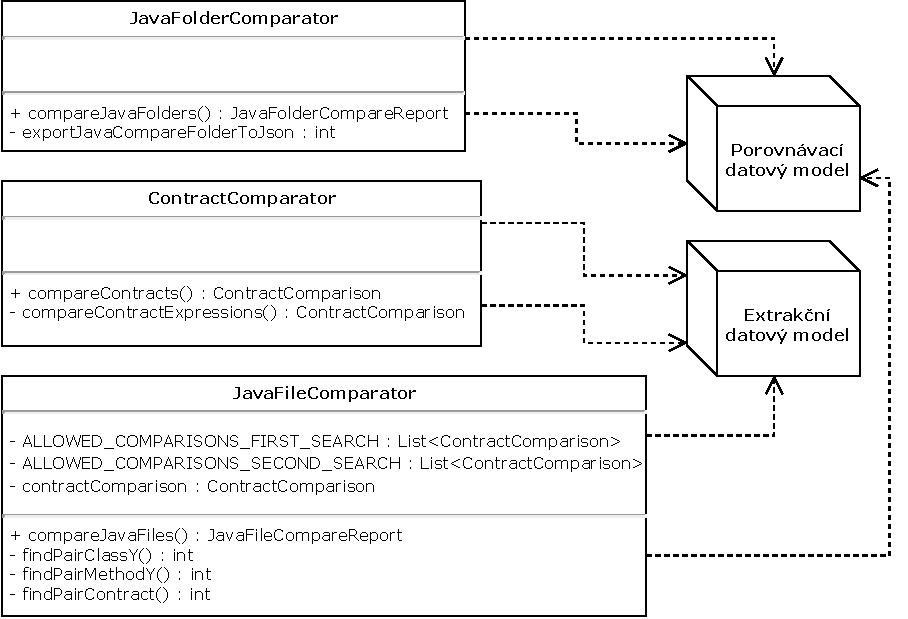
\includegraphics[width=1\textwidth]{img/comparatorUMLdiagram.pdf}
					\caption[comparatorUMLdiagram]{UML diagram porovnávacího modulu}
					\label{comparatorUMLdiagram}
				\endminipage\hfill
			\end{figure}
	    
	    
	    
	    \subsubsection{Porovnávání kontraktů}
	    	Při porovnávání kontraktů se nejprve zkontroluje, zda je shodný typ reprezentace kontraktu, typ podmínky a také funkce. Jestliže je nějaká z těchto položek negativní, kontrakty jsou považovány za rozdílné (\texttt{DIFFERENT} dle výčtového typu \texttt{ContractComparison}). Pokud jsou shodné, je porovnán výraz obou kontraktů. Jestliže je výraz rozdílný, je vrácena hodnota \texttt{DIFFERENT\_EXPRESSION}, pokud ne, zkontrolují se ostatní argumenty. Pokud je některý z nich rozdílný, či je jich rozdílný počet, je vrácena hodnota \texttt{MINOR\_CHANGE}). Pokud byly všechny testované položky v pořádku, je vráceno \texttt{EQUAL}.\\
	    	
	    	Podrobnosti o modelu a jednotlivých hodnotách porovnání byly zmíněny výše v 5.kapitole. Je zde velký prostor pro zlepšení v oblasti porovnávání výrazů, to je více rozebráno níže v kapitole Zhodnocení výsledků.
	    
	    \subsubsection{Porovnávání souborů}
	    	Porovnávání kontraktů v souborech není triviální z důvodu párování jednotlivých kontraktů. Pokud je změněno pořadí kontraktů a změní se jejich definice, je obtížné přiřadit daný kontrakt ke svému protějšku v druhém souboru.\\
	    	
	    	Algoritmus nejprve prochází všechny třídy daného souboru. Pokud se podaří najít shodnou třídu, pokračuje se dále. V opačném případě je přidána do seznamu změn API odebraná třída. Jestliže ale třída byla nalezena, prochází se kontrakty dané třídy (tedy neměnné podmínky).\\
	    	
	    	Párování jednotlivých kontraktů funguje následujícím způsobem. Aktuální kontrakt se hledá v seznamu kontraktů protější třídy, tím že se jednotlivé kontrakty porovnávají. Pokud je výsledkem \texttt{EQUAL} nebo \texttt{MINOR\_CHANGE}, kontrakt je považován za nalezený. V tom případě se přidá záznam o jejich porovnání dle získané hodnoty a kontrakt je vymazán ze seznamu kontraktů protějšku, aby jej nebylo možné znova spárovat. Pokud kontrakt nebyl nalezen, je přidán do seznamu nenalezených kontraktů a hledá se další kontrakt.\\
	    	
	    	Jakmile byly vyhledány všechny kontrakty, prochází se seznam nenalezených kontraktů. Opět se daný kontrakt snažíme vyhledat v seznamu protější třídy, ten je však již redukován. Nyní je shodu považován jakýkoliv výsledek kromě \texttt{DIFFERENT}. Pokud je protějšek nalezen, je považováno, že se kontrakt změnil a je přidán do seznamu porovnání. Pokud kontrakt nebyl nalezen, je předpokládáno, že byl odstraněn a je přidán záznam o odebrání kontraktu.\\
	    	
	    	Toto párování kontraktů je heuristika, při které se může stát, že by se kontrakt spároval s jiným, protože by bylo změněno pořadí kontraktů a zároveň by byly naprosto shodné až na argumenty (tím by se vrátila odpověď \texttt{MINOR\_CHANGE}). Tento scénář je však velmi nepravděpodobný, protože kontrakty, které se liší pouze v ostatních argumentech by byly velice nezvyklé. I v případě, že by tato situace nastala, bylo by možné tuto záměnu poznat ze zprávy, kde by byl dvakrát registrován rozdíl v kontraktech. Vzhledem k tomu, že tyto situace, které mohou nastat jsou vysoce nepravděpodobné, a i když nastanou, je možné je dohledat ve změnách, rozhodl jsem se tuto heuristiku použít. Díky tomu je možné dosáhnout mnohem lepších výsledků, protože není tolik kontraktů považovaných za nenalezené.\\
	    	
	    	Po porovnání neměnných podmínek se prochází jednotlivé metody této třídy. Zde pak probíhá stejný proces jako u párování tříd. Poté se procházejí jednotlivé kontrakty metody. Zde opět funguje stejný princip jako v případě neměnných podmínek.\\
	    	
	    	Následně se zkontroluje, zda některé kontrakty nezbyly v seznamu, pokud ano, jsou registrovány jako nově přidané kontrakty. Metoda je následně vymazána ze seznamu ze stejného důvodu a stejným způsobem jsou ohlášeny všechny metody, které zbyly jako nově přidané. Totéž platí pro třídy a neměnné podmínky. Přidáním jednotlivých záznamů o přidaných/odebraných metodách, třídách a kontraktech (v případě kontraktů také o změněných), jsou vytvořeny seznamy, které pak tvoří závěrečnou zprávu porovnání obou souborů \texttt{JavaFileCompareReport} (viz model výše).
	    
	    \subsubsection{Porovnávání složek}
			Porovnávání složek funguje podobným způsobem jako porovnávání souborů. Respektive stejně jako byly párovány jednotlivé třídy, metody a kontrakty, jsou zde párovány soubory. Je zde tedy také zaznamenáno, které soubory byly přidány a odebrány. Součástí je také seznam jednotlivých zpráv o porovnání souborů. Tím se tvoří \texttt{JavaFolderCompareReport}, který je výsledkem tohoto porovnání.\\
			
			Na rozdíl od předchozího případu je zde nutné nejprve upravit cesty jednotlivých složek, respektive souborů, tak, aby jejich relativní cesta byla shodná.

%%%%%%%%%%%%%%%%%%%%%%%%%%%%%%%%%%%%%%%%%%%%%%%%%%%%%%%%%%%%%%%%%%%%%%%%%%%%%%%%%%%%%%%%%%%%%%%%%%%%%%%%%%%%%%%%%%%%%%%%%%%%%%%%%%%%%%%%%%%%%%%%%%%%%%%%%%%%%%%%%%%%%%%%%%%%%%%%%%%%%%%%    
	    \subsection{API Modul}
	    	Knihovna obsahuje API pro snazší přístup zvnějška. Skládá se z několika částí. Je zde třída \texttt{ApiFactory}, která umožňuje instancování jednotlivých API, jedná se o návrhový vzor továrny. V nástroji jsou definovány celkem čtyři různé typy API, každý z nich implementuje specifické rozhraní, pomocí kterého je možné využít továrny. V nástroji je pouze jedna implementace pro každý typ, továrna a rozhraní jsou zde tedy pouze pro přehlednost a možnost snadného rozšíření.\\
	    	
	    	Zde je seznam všech čtyř typů API podle názvů jejich rozhraní. Implementační třídy pak mají stejný název, ale s přidanou předponou \texttt{Default}:
				
				\begin{itemize}
					\item \texttt{ContractExtractorApi}
					\item \texttt{BatchContractExtractorApi}
					\item \texttt{ContractComparatorApi}
					\item \texttt{BatchContractComparatorApi}
				\end{itemize}					    	
	    	
	    	Následuje stručný výčet toho, co jednotlivá API umožňují. Pro přesný popis metod, jejich parametrů a návratového typu je možné se podívat do JavaDoc projektu.
	    
			\subsubsection{\texttt{ContractExtractorApi}}
					Zde jsou zejména metody pro získání kontraktů. Metoda \texttt{retrieveContracts} umožňuje extrakci kontraktů ze vstupního souboru. Je možné definovat, které typy kontraktů se mají analyzovat a zda mají být vráceny i objekty bez kontraktů. Vrácena je instance \texttt{JavaFile}, která obsahuje extrahované kontrakty. Další metodou je \texttt{retrieveContractsFromFolder}, která poskytuje stejnou funkcionalitu s tím rozdílem, že vstupem je celá složka nikoliv soubor a je vrácen seznam \texttt{JavaFile}.\\
					
					Následně je zde \texttt{exportJavaFilesToJson}. Tato metoda slouží k exportu vstupního seznamu \texttt{JavaFile} do JSON. Je třeba nastavit výstupní složku a také, zda má být formát v minimalistické formě. Poslední metodou pak je \texttt{updateShortPathOfJavaFiles}, která aktualizuje atribut \texttt{shortPath} všech \texttt{JavaFile} v seznamu.	    
			    
			\subsubsection{\texttt{BatchContractExtractorApi}}	
				Toto API poskytuje podobnou funkcionalitu jako předchozí. Obsahuje pouze jednu metodu \texttt{retrieveContractsFromFolderExportToJson}. Jedná se v podstatně o kombinaci předchozích metod. Umožňuje načtení kontraktů z dané složky a jejich následný export do zadaného adresáře, součástí je také shodné nastavení. Tato metoda nejprve načte jeden soubor ten zpracuje, exportuje a pak pokračuje dalším, díky tomu je méně náročná na paměť. Toto API je využito pro konzolovou část uživatelské aplikace.
				
			\subsubsection{\texttt{ContractComparatorApi}}
				Poskytuje metodu \texttt{compareJavaFolders}, která porovná dva zadané adresáře na úrovni kontraktů ale i jejich API. Následně vytvoří report typu \texttt{JavaFolderCompareReport} informující o tomto srovnání. Je možné zvolit, zda se mají reportovat shodné objekty a také jestli se mají reportovat změny API, které přímo neovlivňují kontrakty. Druhou metodou je pak \texttt{exportJavaFolderCompareReportToJson}, což umožňuje vytvořený report exportovat do JSON.
				
			\subsubsection{\texttt{BatchContractComparatorApi}}
				Toto je poslední dostupné API. Opět poskytuje obdobné chování jako předchozí API, s tím rozdílem, že je určeno pro dávkové zpracování a kombinuje obě metody do jedné(\texttt{compareJavaFoldersAndExportToJson}). Tato metoda porovná obě složky a výslednou zprávu následně exportuje do JSON. Stejně jako pro předchozí API tohoto typu i zde platí, že je použito v konzolové části aplikace.
				
			\subsubsection{Použití API}	    
				Použití API je velmi snadné, jak je vidět na následujícím příkladu:\\\\
				\- \- \- \- \- \- \texttt{\textcolor{pgrey}{// Získání instance API pomocí továrny}}\\ 
				\- \- \- \- \- \- \texttt{ApiFactory f = new ApiFactory();}\\
	    		\- \- \- \- \- \- \texttt{ContractExtractorApi api = f.getContractExtractorApi();}\\\\ 
            	\- \- \- \- \- \- \texttt{\textcolor{pgrey}{// Nyní je možné využít metody knihovny}}\\ 
				\- \- \- \- \- \- \texttt{api.retrieveContracts(...);}
	    
%%%%%%%%%%%%%%%%%%%%%%%%%%%%%%%%%%%%%%%%%%%%%%%%%%%%%%%%%%%%%%%%%%%%%%%%%%%%%%%%%%%%%%%%%%%%%%%%%%%%%%%%%%%%%%%%%%%%%%%%%%%%%%%%%%%%%%%%%%%%%%%%%%%%%%%%%%%%%%%%%%%%%%%%%%%%%%%%%%%%%%%%
	    \subsection{Přidání parseru pro nový typ kontraktu}
	    	Při vytváření knihovny i aplikace byl kladen důraz na abstrakci od použitých typů kontraktů, aby bylo možné snadno přidat parser pro nový typ kontraktu. Grafickou aplikaci není třeba nijak měnit, ale je třeba provést několik kroků v rámci knihovny. Pro rozpoznávání nové reprezentace kontraktu jsou potřeba tyto kroky:
	    	
			\begin{enumerate}
				\item Přidání položky do \texttt{ContractType}
				\item Vytvoření nového analyzátoru
				\item Doplnění továrny \texttt{ParserFactory}
				\item Testování
			\end{enumerate}				    	
	    	
	    	\subsubsection{Přidání položky do \texttt{ContractType}}
	    		Nejprve je třeba přidat položku do výčtového typu \texttt{ContractType}. Název by měl být vhodně zvolen, protože je zobrazen v exportovaných datech, ale i v grafické aplikaci. Kontext je dobře vidět na diagramu datového modelu (obrázek \ref{modelExtractorDiagram} v předchozí kapitole).
	    		
	    	\subsubsection{Vytvoření nového analyzátoru}
	    		Následně je třeba vytvořit funkční část daného parseru. Je tedy nutné vytvořit třídu, která bude implementovat rozhraní \texttt{ContractParser}. Toto rozhraní požaduje implementaci pouze jedné metody a tou je \texttt{ExtendedJavaFile retrieveContracts(ExtendedJavaFile extendedJavaFile)}. Aby byly zachovány jmenné konvence současné knihovny, měla by se tato třída jmenovat \texttt{TypXParser}, kde \texttt{TypX} reprezentuje název nového typu kontraktu. Tato třída by se měla nacházet v balíčku se stejným jménem (ale s malými písmeny) a ten by se měl nacházet v balíčku \texttt{cz.zcu.kiv.contractparser.parser}. Tvar samotné metody již závisí na principech daného kontraktu. Obecně platí, že by se měly kontrakty detekovat a vytvořit na základě dat ze vstupního objektu typu \texttt{ExtendedJavaFile} a ve stejném objektu je také vrátit. Pro lepší představu doporučuji prozkoumat již implementované analyzátory pro JSR305 a Guava Preconditions.\\
	    		
	    		Podrobnosti mohou být patrné z diagramu \ref{parserUMLdiagram}, kde jsou zobrazeny všechny zmíněné komponenty. Nový analyzátor by pak byl na úrovni \texttt{GuavaParser} či \texttt{JSR305Parser}.
	    		
	    	\subsubsection{Doplnění továrny \texttt{ParserFactory}} 
	    		Dalším krokem je doplnění továrny \texttt{ParserFactory}. Zde je pouze třeba přidat nový \texttt{case} do konstrukce \texttt{switch}. Tento blok by měl vracet instanci nového parseru v případě že vstoupí tento typ v objektu \texttt{ContractType}.
	    			
	    	\subsubsection{Testování}
	    		Pro bezchybnou funkci daného analyzátoru je možné vytvořit jednotkové testy. Testovací data pro současné testy jsou umístěny v \texttt{resources/testFiles}, kde jsou pak dále děleny do složek.

    
    
    
    
%%%%%%%%%%%%%%%%%%%%%%%%%%%%%%%%%%%%%%%%%%%%%%%%%%%%%%%%%%%%%%%%%%%%%%%%%%%%%%%%%%%%%%%%%%%%%%%%%%%%%%%%%%%%%%%%%%%%%%%%%%%%%%%%%%%%%%%%%%%%%%%%%%%%%%%%%%%%%%%%%%%%%%%%%%%%%%%%%%%%%%%%
%%%%%%%%%%%%%%%%%%%%%%%%%%%%%%%%%%%%%%%%%%%%%%%%%%%%%%%%%%%%%%%%%%%%%%%%%%%%%%%%%%%%%%%%%%%%%%%%%%%%%%%%%%%%%%%%%%%%%%%%%%%%%%%%%%%%%%%%%%%%%%%%%%%%%%%%%%%%%%%%%%%%%%%%%%%%%%%%%%%%%%%%
%%%%%%%%%%%%%%%%%%%%%%%%%%%%%%%%%%%%%%%%%%%%%%%%%%%%%%%%%%%%%%%%%%%%%%%%%%%%%%%%%%%%%%%%%%%%%%%%%%%%%%%%%%%%%%%%%%%%%%%%%%%%%%%%%%%%%%%%%%%%%%%%%%%%%%%%%%%%%%%%%%%%%%%%%%%%%%%%%%%%%%%%
%%%%%%%%%%%%%%%%%%%%%%%%%%%%%%%%%%%%%%%%%%%%%%%%%%%%%%%%%%%%%%%%%%%%%%%%%%%%%%%%%%%%%%%%%%%%%%%%%%%%%%%%%%%%%%%%%%%%%%%%%%%%%%%%%%%%%%%%%%%%%%%%%%%%%%%%%%%%%%%%%%%%%%%%%%%%%%%%%%%%%%%%
	\section{Uživatelská aplikace}
	   \subsection{Použité technologie}
	    	 Aplikace byla, stejně jako knihovna, implementována v jazyce Java verze 1.8 ve vývojovém prostředí IDEA IntelliJ Ultimate 2017.3.3 s využitím Apache Maven. Grafické uživatelské rozhraní bylo vytvořeno využitím platformy JavaFX. 
	    	 
	    	 \subsubsection{Externí knihovny}
				Mimo následujících knihoven byly opět využity externí knihovny Apache Log4j a Google Gson, které byly popsány výše.
			
			\paragraph{ControlsFX} 
				Tato knihovna rozšiřuje JavaFX a umožňuje použití dalších funkcí a objektů zejména pak \texttt{CheckListView}, což je použito pro zobrazení seznamu souborů \cite{controlsfx}. 
			
			\paragraph{FontAwesomeFX} 	
				Knihovna FontAwesomeFX slouží opět k rozšíření JavaFX. Tuto knihovnu jsem použil pro rozšíření možností zobrazení ikon \cite{fontawesomefx}.	 
		
		\subsection{Design grafické části aplikace}
			Grafická část aplikace byla rozdělena na dvě části dle její funkčnosti. První z nich je extrakční, ta umožňuje extrakci kontraktů ze souborů a jejich následný export. Také je možné prohlížet si podrobnosti o jednotlivých souborech.  Druhá část slouží k porovnávání kontraktů. Mezi těmito částmi je možné přepínat pomocí záložky.\\
			
			Každá část disponuje panelem nástrojů, pomocí kterého je možné přidávat, mazat a exportovat označené soubory. Dále je zde panel filtrů, kde lze nastavit různé podrobnosti ohledně zobrazených dat. Obě části také mají seznam souborů, kde jsou zobrazeny všechny soubory, které byly přidány (může být ovlivněno filtry). Jednotlivé soubory pak mohou být označeny pro výše zmíněné mazání a export. Součástí obou částí jsou také globální statistiky, které zobrazují různé podrobnosti a shrnutí vybraných souborů. Vidět je také detail právě vybraného souboru. Zde je možné zobrazit si podrobnosti a otevřít tak nové okno aplikace, kde jsou detailní informace o daném souboru, včetně stromové reprezentace daného souboru.\\
			
			Tato sekce představuje pouze krátké shrnutí toho, jak je aplikace členěna a co umožňuje pro pochopení kontextu. Pro podrobnější popis je možné nahlédnout do přílohy A Uživatelská příručka, kde jsou podrobně vysvětleny všechny funkce za pomoci obrázků aplikace.
		
		\subsection{Struktura aplikace}
			Uživatelská aplikace je rozdělena do několika částí dle balíčků v projektu. Prvním z těchto balíčků je \texttt{application}, který má na starosti uchování dat aplikace, jako jsou data seznamů souborů, statistiky, aktuálně vybraný soubor atd. Jsou zde také nastavovány různé funkce pro dané objekty, které jsou vykonávány na základě vnějších podnětů. Příkladem může být aktualizace dat, přidávání souborů do seznamu atd.\\
			
			Další částí je \texttt{controller}, kde se nachází ovládací prvek, jež definuje akce po stisknutí tlačítek . Zde jsou typicky volány akce definované v části \texttt{application}.\\
			
			Následuje část \texttt{utils}, která poskytuje různé funkce jako je práce se zdroji, práce se soubory, ale také je zde definována konzolová část aplikace.\\
			
			Mimo tyto balíčky je zde také třída \texttt{ContractManager}, která představuje hlavní třídu celé aplikace a definuje její spuštění. Kontroluje, zda se má aplikace spustit v grafickém režimu či jen vykonat daný příkaz. Je zde také definováno okno a scéna grafické části.\\
			
			Následuje stručný popis jednotlivých balíčků a jejich důležitých tříd. Další podrobnosti je pak možné nalézt ve vygenerované dokumentaci JavaDoc.
					 
			
			\subsubsection{Balíček \texttt{application}}
				Nachází se zde třída \texttt{Settings}, která uchovává nastavení filtrů aplikace. Potenciálně je tuto část možné rozšířit o další nastavení, které by mohlo měnit chování či vzhled aplikace. Hlavní třídou balíčku je pak \texttt{ApplicationData}. Ta obsahuje data obou záložek i zmíněné nastavení, jedná se o přístupový bod ke zbytku aplikace. Samotné záložky jsou pak definovány dvěma třídami \texttt{ExtractorApplicationTab} a \texttt{ComparatorApplicationTab}. Ty obě dělí od obecné třídy \texttt{ApplicationTab}. Každá z těchto tříd také obsahuje třídu \texttt{ExtractorFileList} respektive \texttt{ComparatorFileList}, které obsahují detaily o seznamech souborů včetně samotných souborů.
				
			\subsubsection{Balíček \texttt{controller}}
				Tento balíček je poměrně přímočarý a obsahuje pouze jedinou třídu \texttt{Controller}. Zde jsou pak mapovány metody na jednotlivá stisknutí tlačítek.
		
			\subsubsection{Balíček \texttt{utils}}
				Třída \texttt{ConsoleApplication} představuje konzolovou část aplikace. Zde probíhá zpracování vstupních parametrů a jejich následné předání patřičným metodám. Jsou zde také ošetřeny chybné vstupy a nastavení chybových zpráv.\\
				
				Dále je zde třída \texttt{FileHandler}, která má na starosti výběr souborů také jejich export.\\
				
				Pomocí třídy \texttt{ResourceHandler} je pak možné přistupovat ke zdrojům, které obsahují nastavitelné vlastnosti \texttt{properties} a také lokalizované texty uživatelského rozhraní spolu s chybovými a informačními hláškami. Texty jsou k dispozici pouze v angličtině, ale díky přístupu pomocí zdrojů je možné snadno přidat další jazyky.\\
				
				Samotná třída \texttt{Utils} pak obsahuje pomocné metody pro snazší vyhledávání prvků v rozhraní, centrování okna na obrazovku atd.		
		
	    	   
	   \subsection{Ovládání aplikace}
	   		Pro zlepšení práce s aplikací, byla rozdělena na dvě části. Aplikaci je možné spustit bez parametrů jako grafickou aplikaci, případně je možné aplikaci spustit s parametry, čímž se provede jednorázová akce pro dávkové zpracování. Podrobné informace o spouštění a používání aplikace jsou uvedeny v příloze A. Uživatelská příručka.
	   		
	   		\subsubsection{Grafická část}
	   			Standardním spuštěním aplikace bez parametrů se zobrazí grafická uživatelská část. Zde je možné extrahovat kontrakty, zobrazovat si je v kontextu hierarchie daného souboru, exportovat získaná data a také porovnávat složky za účelem zjištění rozdílů v API a kontraktech. Všechny tyto činnosti je možné obsluhovat pomocí jednoduchého a intuitivního uživatelského rozhraní.			   			  		
	   		\subsubsection{Konzolová část}
	   			V případě, že chceme pouze provést jednorázovou akci extrakce či porovnávání kontraktů a následný export, je možné využít konzolové části aplikace, tedy spustit aplikaci s příslušnými parametry (viz Uživatelská příručka). Takto je možné snadno a rychle provádět dávkové operace. Tento způsob zpracování je také méně náročný na paměť zařízení.
	   
	   \subsection{Možnosti a limitace aplikace}
	   		Při vývoji uživatelské aplikace byl kladen důraz na snadné a intuitivní použití, které poskytne možnost jak vyzkoušet a aktivně využít vytvořenou knihovnu. Nástroj je určen pro výzkumné účely uzavřené skupiny, nikoliv pro použití širší veřejností. Z tohoto důvodu nebyl kladen důraz na její široké možnosti a uživateli může připadat, že postrádá prvky, které jsou typické pro komerční aplikace. Příkladem může být perzistence dat, široké možnosti filtrování a řazení, propojení s externími editory atd. Níže, v podkapitole Prostor pro zlepšení, je této problematice věnována větší část.




%%%%%%%%%%%%%%%%%%%%%%%%%%%%%%%%%%%%%%%%%%%%%%%%%%%%%%%%%%%%%%%%%%%%%%%%%%%%%%%%%%%%%%%%%%%%%%%%%%%%%%%%%%%%%%%%%%%%%%%%%%%%%%%%%%%%%%%%%%%%%%%%%%%%%%%%%%%%%%%%%%%%%%%%%%%%%%%%%%%%%%%%
%%%%%%%%%%%%%%%%%%%%%%%%%%%%%%%%%%%%%%%%%%%%%%%%%%%%%%%%%%%%%%%%%%%%%%%%%%%%%%%%%%%%%%%%%%%%%%%%%%%%%%%%%%%%%%%%%%%%%%%%%%%%%%%%%%%%%%%%%%%%%%%%%%%%%%%%%%%%%%%%%%%%%%%%%%%%%%%%%%%%%%%%
%%%%%%%%%%%%%%%%%%%%%%%%%%%%%%%%%%%%%%%%%%%%%%%%%%%%%%%%%%%%%%%%%%%%%%%%%%%%%%%%%%%%%%%%%%%%%%%%%%%%%%%%%%%%%%%%%%%%%%%%%%%%%%%%%%%%%%%%%%%%%%%%%%%%%%%%%%%%%%%%%%%%%%%%%%%%%%%%%%%%%%%%
%%%%%%%%%%%%%%%%%%%%%%%%%%%%%%%%%%%%%%%%%%%%%%%%%%%%%%%%%%%%%%%%%%%%%%%%%%%%%%%%%%%%%%%%%%%%%%%%%%%%%%%%%%%%%%%%%%%%%%%%%%%%%%%%%%%%%%%%%%%%%%%%%%%%%%%%%%%%%%%%%%%%%%%%%%%%%%%%%%%%%%%%	   
\section{Optimalizace}
	I přesto, že efektivita nebyla prioritou tohoto projektu, v rámci možností jsem se snažil obě části nástroje zanalyzovat a následně optimalizovat. Díky tomu se mi podařilo zpřehlednit kód, odhalit řadu chyb, snížit nároky na paměť i zrychlit různé algoritmy.

	\subsection{Analýza a refaktoring kódu}
		V průběhu projektu jsem kód analyzoval kvůli potenciálním možnostem vylepšení a odstranění chyb. To vedlo k refektorování nepřehledných či špatně navržených úseků kódu a v důsledku toho jsem snížil cyklomatičnost některých algoritmů a zpřehlednil kód. Díky tomu jsem také odstranil řadu chybu jako jsou neinicialziované proměnné, nekontrolované přetypování atd.\\
		
		Tuto analýzu jsem prováděl ručně, ale také za pomoci nástrojů vývojového prostředí, které poskytují řadu způsobů, jak zkvalitnit kód. 
  	
	\subsection{Zjednodušení modelu} 
		V rámci optimalizace jsem také zjednodušil datový model. Ten původní obsahoval komplexní objekty vytvořené knihovnou JavaParser, což vedlo k vyšším nárokům na paměť a snižovalo to celkovou přehlednost kódu, ale také exportovaných dat. V původním modelu jsem také uchovával informace jako těla metod a anotace, která již nejsou ve finálním modelu potřebná, což opět vedlo ke snížení přehlednosti a zvýšení paměťové náročnosti. Na základě toho vznikly pomocné třídy \texttt{extendedJavaFile/Class/Method}, které umožňují uchování důležitých dat pouze během analýzy.
 
	\subsection{Snížení nároků na paměť pro dávkové zpracování}
		Ve své původní verzi, konzolová část uživatelské aplikace využívala stejné API jako část grafická. Proto byly dávkové operace zpracovávány tak, že se nejprve všechny položky načetly do paměti a teprve poté byly exportovány. To samozřejmě bylo zbytečně náročné na paměť, protože v dávkovém zpracování není třeba průběžně uchovávat analyzované soubory. Z tohoto důvodu vznikla nová API a metody, které umožňují průběžné zpracování bez zbytečného zatížení paměti.
